\section{The Human Visual System}
\label{sec:HVS_attention}

\subsection{The Human Visual System}

% ADD VERY short anatomy section

A simplified model estimates the field of view to be approximately 200° to 220° horizontally and around 125° vertically, with the vertical field of view extending slightly further downward [\cite{loschkyScenePerceptionCentral2017}]. The central vision covers about 5° around the point of fixation, where acuity is highest [\cite{loschkyScenePerceptionCentral2017}, \cite{rosenholtzCapabilitiesLimitationsPeripheral2016}]. The remaining field is the periphery, with boundaries at 30° and 60°, dividing it into near, mid and far peripheral vision.

\begin{figure}[hbt]
    \centering
    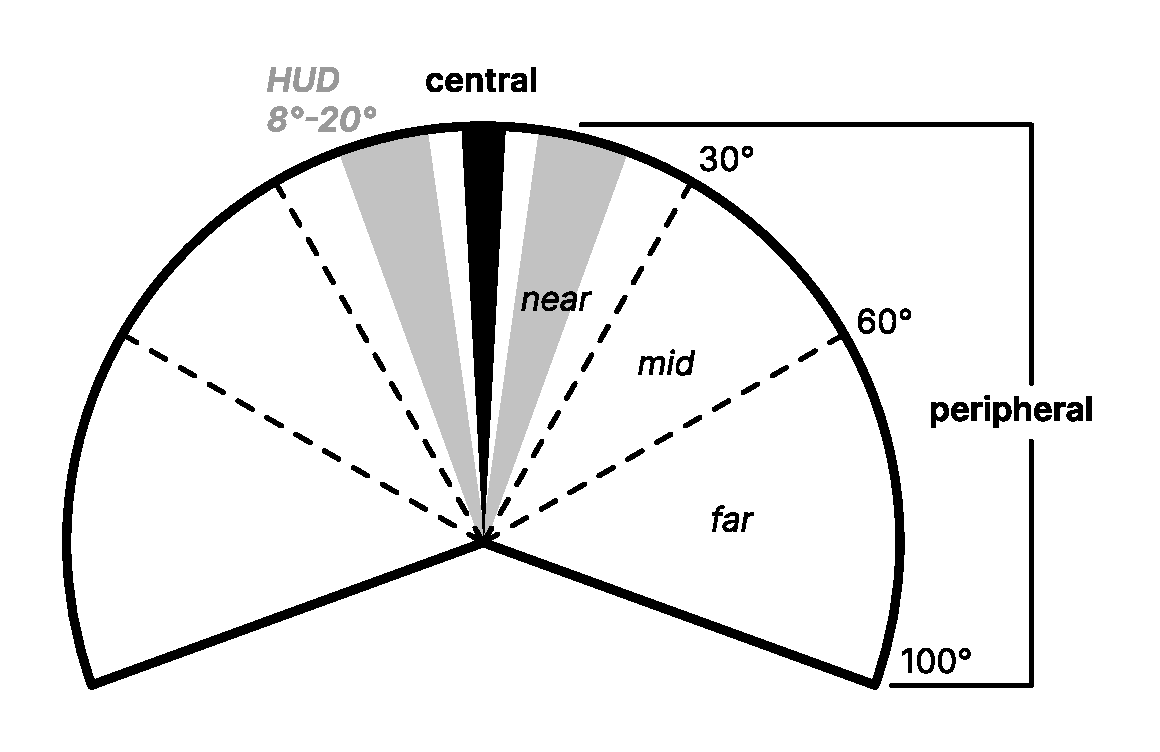
\includegraphics[width=0.5\textwidth]{assets/FOV.eps}
    \caption{Simplified illustration of the horizontal field of view.}
    \label{fig:FOV}
\end{figure}

%Despite changing anatomical structure from central field of vision to the periphery, 
Despite visual acuity and other functions deteriorating in the periphery, the area in front of us continues to appear in high resolution, with high contrast and color saturation [\cite{loschkyScenePerceptionCentral2017}]. According to \textcite{rosenholtzCapabilitiesLimitationsPeripheral2016} the decline in performance of the peripheral vision is smaller than commonly assumed. A scene does not require many details to still allow object recognition and orientation, which is why image thumbnails remain recognizable despite their small size.

\textcite{rosenholtzCapabilitiesLimitationsPeripheral2016} suggests that crowding is the biggest issue in parsing information located in the periphery. The effect is more pronounced if the target and its neighboring elements are similar (e.g., same color and shape) [\cite{pelliUncrowdedWindowObject2008}]. The farther elements are from the center of vision, the greater the distance between them must be.

% GRAPHIC include fig 4 of ROSENHOLTZ 1016? The letters placed close together are perceived as one unit rather than three.
% \cite{pelliUncrowdedWindowObject2008} has a lot of examples

In addition, peripheral vision is particularly well suited for detecting motion, provides better vision in low-light conditions [\cite{johnsonChapter5Our2014}] and contributes to functions like orientation, navigation, balance, and hand-eye coordination. A restriction of the peripheral visual field severely impairs the performance of these functions, the effect increasing with the amount of vision obstructed [\cite{alfanoRestrictingFieldView1990}].

Color sensitivity decreases toward the periphery, red-green moreso than blue-yellow colors and sensitivity to luminance. \textcite{hansenColorPerceptionIntermediate2009} found that color perception is possible even at an eccentricity of 50°, provided the stimulus is sufficiently large. Most modern OST-HMDs feature a 40° field of view, meaning the entire available color spectrum can be utilized.

\subsection{Visual Attention}

The retina transmits too much information to be processed all at once. This bottle neck is resolved by visual attention—by limiting processing to focus on just a fragment of the current visual stimuli [\cite{andersonDirectedVisualAttention2005}, \cite{rosenholtzCapabilitiesLimitationsPeripheral2016}]. This process is guided by peripheral vision, which subconsciously preselects salient features of the environment [\cite{}]. Visual salience describes features that distinguish a target from its surrounding objects [\cite{johnsonChapter5Our2014}].
% -> visual hierarchy
% -> non-linear visual search

% \cite{rosenholtzCapabilitiesLimitationsPeripheral2016}
% - “Because of the brain's limited capacity, our visual systems cannot automatically perform every possible visual task at the same time. Instead, the brain may concentrate resources on one task in a given moment, then switch to focus on another task.”
% - “Our results suggest that the visual system looks for evidence of a change throughout the visual field, possibly in parallel, rather than looking for a change merely where one fixates. However, that evidence of a change can be weak because of loss of information in peripheral vision, making change detection difficult.”

% \cite{caterSelectiveQualityRendering2002}
% - process by which we humans select a portion of the available visual information for localization, identification, and understanding of objects in an environment
% - allows the visual system to process visual input preferentially by shifting attention about an image, giving more attention to salient locations and less attention to unimportant regions

% GRAPHIC perception pipeline: perception, attention as filter, cognition

% Saccades: fast, scanning movements, Fixations: eye focuses on one spot to comprehend, metrics for attention: fixation duration, frequency